\documentclass{emulateapj}
%\documentclass[manuscript]{aastex}

\usepackage{graphicx}
\usepackage{subfigure}
\usepackage{verbatim}
\usepackage{natbib}
\usepackage{amsmath}
\usepackage{color}
\bibliographystyle{apj}

\shorttitle{STAR-FORMING MAIN SEQUENCE GALAXIES AND THEIR MORPHOLOGY}
\shortauthors{WILLETT ET AL.}

\newcommand{\mytilde}{\raise.17ex\hbox{$\scriptstyle\mathtt{\sim}$}}
\newcommand{\kevin}{{\color{red}\textbf{Kevin}}}

\begin{document}

\title{The dependence of spiral disk morphology on the star formation-stellar mass relation}

\author{Kyle Willett\altaffilmark{1}, Kevin Schawinski\altaffilmark{2}, etc.}

\altaffiltext{1}{School of Physics and Astronomy, University of Minnesota, Minneapolis, MN 55455, USA}
\altaffiltext{2}{Institute for Astronomy, Department of Physics, ETH Z\"urich, Wolfgang-Pauli-Strasse 16, CH-8093, Z\"urich, Switzerland}

% Hello, @overheardonastroph!

%%%%%%%%%%%%
%%% ABSTRACT
%%%%%%%%%%%%

\begin{abstract}
We measure the mass-star formation relation in disk galaxies at $z<0.05$, using Galaxy Zoo morphologies to examine different populations of spirals as classified by their kiloparsec-scale structure. We examine the number of spiral arms, their average pitch angle, and the presence of a galactic bar in the disk, and show that both the slope and dispersion of the $M_\star$-SFR relation is constant when varying all the above parameters. We also show that mergers (both major and minor), which represent the strongest conditions for increases in star formation at a constant mass, only drive the galaxies off the main relation by $\sim0.3$~dex; this is a significant reduction over the increase seen in merging systems at $z>1$. Of the galaxies lying significantly above the $M_\star$-SFR relation in the local Universe, more than $50\%$ are mergers. We interpret this as evidence that the spiral arms, which are imperfect reflections of the galaxy's current gravitational potential, are either fully independent of the basic quenching relation or are completely overwhelmed by the combination of outflows and feedback. The arrangement of the star formation can be changed (as demonstrated by the filling factor of the disk), but the system \emph{as a whole} regulates itself even in the presence of strong dynamical forcing. 
\end{abstract}

\keywords{galaxies:mergers}

%%%%%%%%%%%%
%%% INTRODUCTION
%%%%%%%%%%%%

\section{Introduction} \label{sec-intro}

Observations at a range of redshifts have established that the star formation rate (SFR) of a galaxy is strongly correlated to its stellar mass ($M_\star$). This ``star-forming main sequence'' (SFMS) is nearly linear and at least at low redshift, has remarkably small scatter \citep{bri04}. Recent observations of star-forming galaxies at high redshifts show that this main sequence remains out to high redshift, but with its normalisation shifting up so that galaxies of the same $M_\star$ have a higher SFR at high redshift \citep{noe07,dad07}. The main sequence has been interpreted by \citet{bou10} and \citet{lil13} as the result of the balancing of inflows of cosmological gas and outflows due the feedback. Galaxies self-regulate to remain in a state of homeostasis as they convert baryons from gas to stars. 

As star-forming galaxies exhibit a wide range of physical appearances in optical images, we can ask the natural question of whether the specifics of this physical appearance, and its underlying dynamical processes, have any effect on this homeostasis and therefore the galaxy's location relative to the SFMS. If the details of a galaxy's physical appearance are correlated with position relative to the main sequence, then the dynamical processes that give rise to them -- such as bar formation and spiral arm pitch angle -- are a fundamental aspect of the galaxy's regulatory mechanism. If, on the other hand, these features are not correlated, then there are two options: either galaxy substructure is simply not relevant to the overall $M_\star$-SFR relationship, or the regulatory mechanism overcomes the local effect of substructure in all circumstances. This ultimately relates to the physical processes that control the overall strength of the regulator in each galaxy.

Discuss (\kevin) seminal work of \citet{pen10a,pen12,pen14a,pen14} on gas regulator model and how mass/environment drive galaxy evolution. 

In this paper, we use the Sloan Digital Sky Survey \citep{yor00,str02,aba09} in combination with the largest database of visual classifications of galaxy structure and morphology ever assembled from the Galaxy Zoo citizen science projects \citep{lin08,lin11,wil13} to test whether galaxy structure affects their star formation properties.

%%%%%%%%%%%%
%%% Data
%%%%%%%%%%%%

\section{Data} \label{sec-data}

Data for all galaxies in this paper comes from optical observations in the SDSS~DR7. The morphological data is drawn from citizen science classifications in Galaxy~Zoo. Merging pairs of galaxies are taken from the catalog of \citet{dar10a}, all of which lie in the redshift range $0.005<z<0.1$. Post-merger spheroidal galaxies without an obvious, separated companion are specifically excluded from the sample. Detailed classifications of disk morphologies, including arm pitch angle, number of spiral arms, and presence of a galactic bar, are taken from the Galaxy~Zoo~2 (GZ2) catalog \citep{wil13}. 

Spiral galaxies are selected according to the following thresholds in the spectroscopic GZ2 sample, where $p$ is the debiased vote fraction and $N$ the weighted number of total votes: $p_\textrm{features/disk} > 0.430$, $p_\textrm{not~edgeon} > 0.715$, $p_\textrm{spiral}>0.619$, and $N_\textrm{spiral}>20$. We identify sub-classes of spiral structure using the morphology flags as given in the GZ2 catalog; these are designed to be conservative cuts, including only robust examples of each morphological class. 

Stellar masses and star formation rates are computed from optical diagnostics and taken from the MPA-JHU catalogue \citep{kau03a,bri04}. We use updated masses and activity classifications from the DR7 database.\footnote{\url{http://home.strw.leidenuniv.nl/\mytilde jarle/SDSS/}} We separate star-forming galaxies from other emission-line galaxies using the standard BPT classification \citep{bal81} below the \citet{kau03} demarcation. Galaxies with low signal-to-noise ratio $(S/N > 3)$ galaxies are removed. For both $M_\star$ and $SFR$, we use median values extracted from the PDF.

%How many galaxies are there in the total sample? What is the mass, color, and redshift range?
The total sample analyzed contains 52,685 star-forming galaxies. These are selected from the GZ2 spectroscopic sample with $z<0.1$, $M_r<-19.5$, and classified as actively star-forming ($BPT=1$) from the MPA-JHU emission line measurements. The average color for the star-forming galaxies is relatively blue, with $(u-r)=1.7\pm0.6$. 

\begin{table} \caption{Basic properties of the $M_\star-SFR$ linear fit for GZ2 star-forming galaxies.}
 \begin{tabular}{@{}lrcrcl}
 \hline
\multicolumn{1}{c}{Sample} &
\multicolumn{1}{c}{$N$} &
\multicolumn{1}{c}{$\alpha$} &
\multicolumn{1}{c}{$\beta$} &
\multicolumn{1}{c}{$\sigma_\alpha$} &
\multicolumn{1}{c}{$\sigma_\beta$} 
\\ 
\hline
\hline						
SF galaxies  & 52685   & $0.73$  & $-7.19$   & $5.27\times10^{-6}$  & $5.18\times10^{-4}$  \\
\hline
1 arm        & 39      & $0.66$  & $-6.31$  &  $5.11\times10^{-3}$  & $5.14\times10^{-1}$  \\
2 arms       & 2914    & $0.79$  & $-7.74$  &  $1.11\times10^{-4}$  & $1.14\times10^{-2}$  \\
3 arms       & 89      & $0.57$  & $-5.47$  &  $4.17\times10^{-3}$  & $4.49\times10^{-1}$  \\
4 arms       & 9       & $0.35$  & $-3.29$  &  $9.18\times10^{-2}$  & $9.58\times10^{0 }$  \\
5+ arms      & 9       & $0.64$  & $-6.88$  &  $7.20\times10^{-2}$  & $6.91\times10^{0 }$  \\
can't tell   & 40      & $0.69$  & $-7.10$  &  $1.06\times10^{-2}$  & $1.04\times10^{0 }$  \\
\hline
tight arms   &  308    & $0.73$  & $-7.26$  &  $1.68\times10^{-3}$  & $1.75\times10^{-1}$  \\
medium arms  &  44     & $0.80$  & $-7.83$  &  $5.23\times10^{-3}$  & $5.37\times10^{-1}$  \\
loose arms   &  470    & $0.74$  & $-7.14$  &  $5.16\times10^{-3}$  & $5.18\times10^{-2}$  \\
\hline
barred       &  4473   & $0.76$  & $-7.54$  &  $7.60\times10^{-5}$  & $7.57\times10^{-3}$  \\
unbarred     &  11593  & $0.70$  & $-6.92$  &  $2.65\times10^{-5}$  & $2.66\times10^{-3}$  \\
\hline
merger       &  2978   & --      & $-7.91$  &  --                   & $4.40\times10^{-4}$  \\
\hline
 \end{tabular}
\tablecomments{Parameters $\alpha$ and $\beta$ are fit according to Equation~\ref{eqn-linearfit}.\label{tbl-fits}}
\end{table}

To parametrize the $M_\star-SFR$ relationship, we apply a simple linear model for the total sample and subsamples. We apply a least-squares fit where the data are weighted by the uncertainty in SFR (computed as the mean difference in the 16th and 84th percentiles from the MPA-JHU PDFs). The data are then fit to:

\begin{equation}
\log(SFR) = \alpha(\log[M_\star/M_\odot]) + \beta \hspace{20pt}[M_\odot/yr]
\label{eqn-linearfit}
\end{equation}

\noindent where $\alpha$ and $\beta$ represent the slope and offset, respectively. Values of the fits for each subample are given in Table~\ref{tbl-fits}; we also provide the formal uncertainties $\sigma_\alpha$ and $\sigma_\beta$ in each parameter from the covariance matrix.

%%%%%%%%%%%%
%%% RESULTS
%%%%%%%%%%%%

\section{Results} \label{sec-results}

We analyze the dependence of the star-forming main sequence for three different sets of disk galaxies: splitting the sample by the observed number (multiplicity) of spiral arms, the relative pitch angle (tightness or winding) of the spiral arms, and the presence of a galactic bar. Both spiral arms and galactic bars can have significant effects on the local properties of a galaxy. Dynamical effects compress gas and trigger recent star formation within spiral arms, while longer galactic bars have redder colors and less star formation than the rest of the disk \citep{hoy11}. We examine whether these kpc-scale effects can be seen long-term in the galaxy's SFR-mass relationship. 

For a control sample, we plot in Figures~\ref{fig-number}-\ref{fig-mergers} the underlying star-forming main sequence relation for star-forming disks as measured in a sample of local SDSS galaxies. As demonstrated in previous papers, there is a fairly tight correlation between $M_\star$ and SFR, with galaxies in the process of quenching lowering their SFR and falling below the trend. The relationship extends over at least 4~orders of magnitude in both $M_\star$ and SFR. 

\begin{figure*}
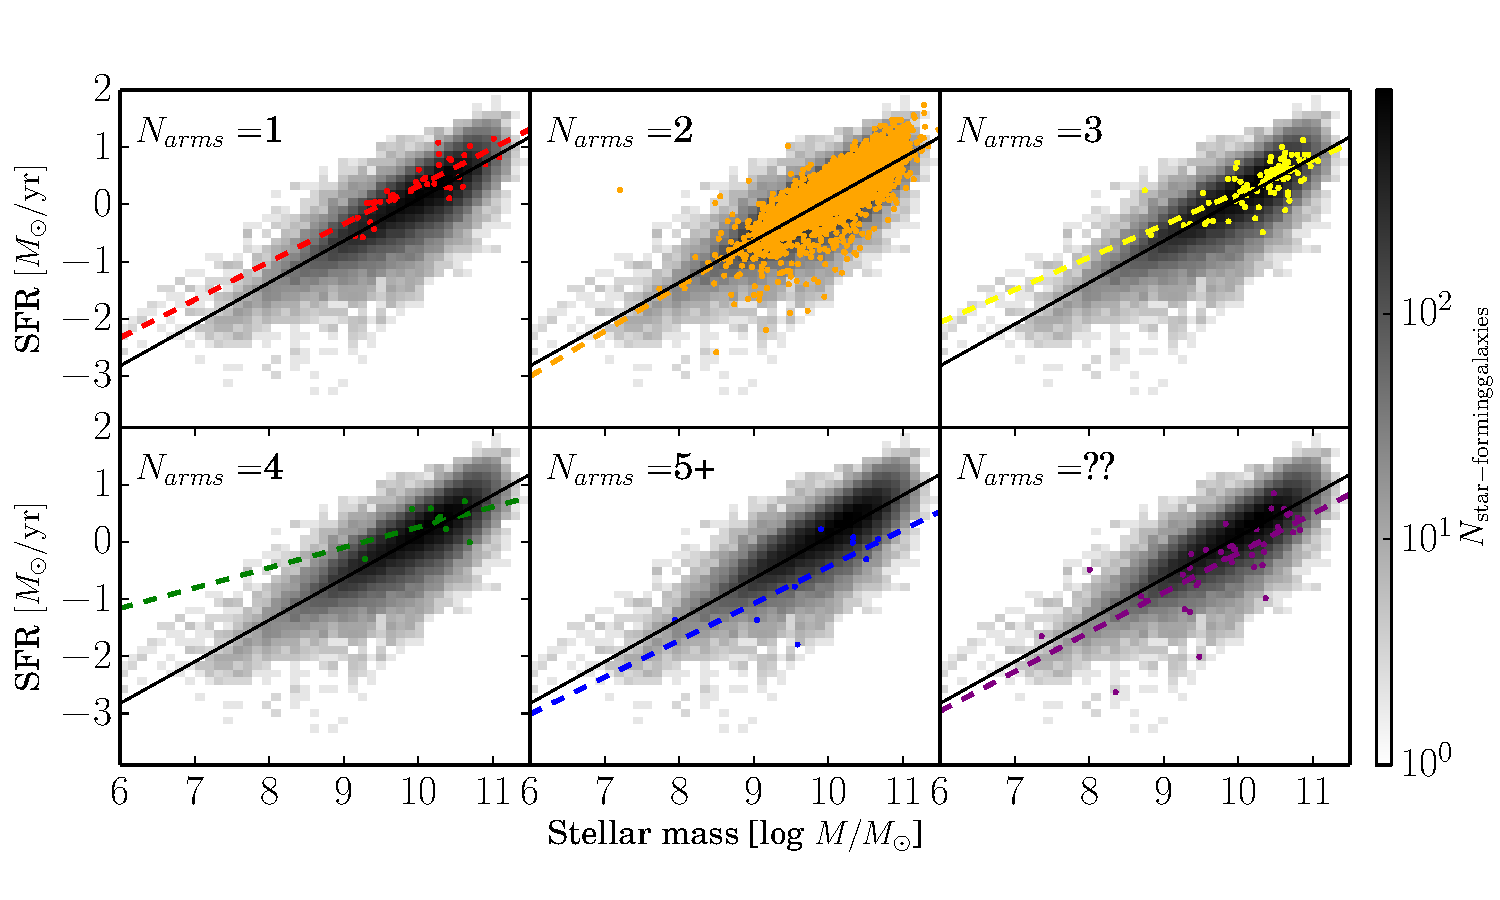
\includegraphics[angle=0,width=7.0in]{figures/ms_arms_number.pdf}
\caption{Total star formation rate as a function of stellar mass; grayscale colors are the distribution of all star-forming galaxies in SDSS from the MPA-JHU DR7 catalog. Colored points in each panel show spiral galaxies with 1, 2, 3, 4, more than four, or ``uncertain'' numbers of spiral arms per galaxy, as identified by GZ2 morphology flags. Dotted lines show the weighted least-squares linear fit to each population as split by arm multiplicity; the solid line is the fit to all of the star-forming galaxies. 
\label{fig-number}}
\end{figure*}

Figure~\ref{fig-number} overplots SFR as a function of $M_\star$ for disk galaxies separated by their arm multiplicity. The GZ2 data separates disk galaxies with visible spiral arms into categories of 1, 2, 3, 4, or more than four spiral arms; there is also an additional option if the number of spiral arms cannot be accurately determined. There are a total of 14,179 galaxies with flags for arm multiplicity (indicating a high level of agreement among classifiers) in the GZ2 data. Of those, two-armed spirals are by far the most common, comprising 85\% of the total. This is also the only multiplicity for which significant numbers of galaxies at $M_\star<10^9~M_\sun$ are detected. 

The fit to the star-forming main sequence for two-armed spirals tighly follows that of that for all spiral galaxies, with both the slope and offset of the linear fits completely consistent with each other (Table~\ref{tbl-fits}). Similarly, the fits for 3, 4, and $5+$-armed spirals are also consistent with the main relation (although all three have much lower numbers which affect the quality of the fit). 

The one-armed spirals present an interesting case, with the majority of the population lying slightly above the fit to all star-forming spirals. This is consistent with the work of \citet{cas13}, who showed that one-armed spirals in GZ2 are robust indicators of close interactions at projected distances of $r_p < 50~h^{-1}$~kpc. The underlying reason is that many ``one-armed spirals'' are in fact caused by bridges or tidal tails from interactions with a nearby companion; we discuss the likely role of merging/interacting galaxies in Figure~\ref{fig-mergers}. 

Finally, galaxies with an uncertain number of spiral arms (although also with relatively low numbers) fall slightly below the mean star-forming main sequence relation. One possibility is that this is a consequence of galaxies that have already begun the process of quenching. As a result, the star-formation rate is depleted and the contrast of spiral arms against the rest of the disk (which for visual identification is at least in part dependent on bright knots of recent star formation) makes the multiplicity more difficult to identify. However, the $(u-r)$ colors of these galaxies (uncorrected for dust extinction) are on average significantly bluer than green-valley late-types as identified in \citet{sch14}.

The pitch angle of the spiral arms also has no significant change on the star-forming main sequence relation (Figure~\ref{fig-winding}). We separate galaxies by their relative pitch angles (defined as ``tight'', ``medium'', and ``loose''); the pitch angle is typically used as one of the primary drivers for separating galaxies along the Hubble tuning fork. \citet{wil13} show, however, that pitch angle only weakly correlates with Hubble type from expert visual classifications, and that the bulge-to-disk ratio is a more important driver. All three categories correlate tightly with spiral galaxies in general; we note that the small deviation above the main sequence for loosely-wound galaxies is also consistent with \citet{cas13}, who show that this morphology also correlates with close pairs and interactions. 

\begin{figure*}
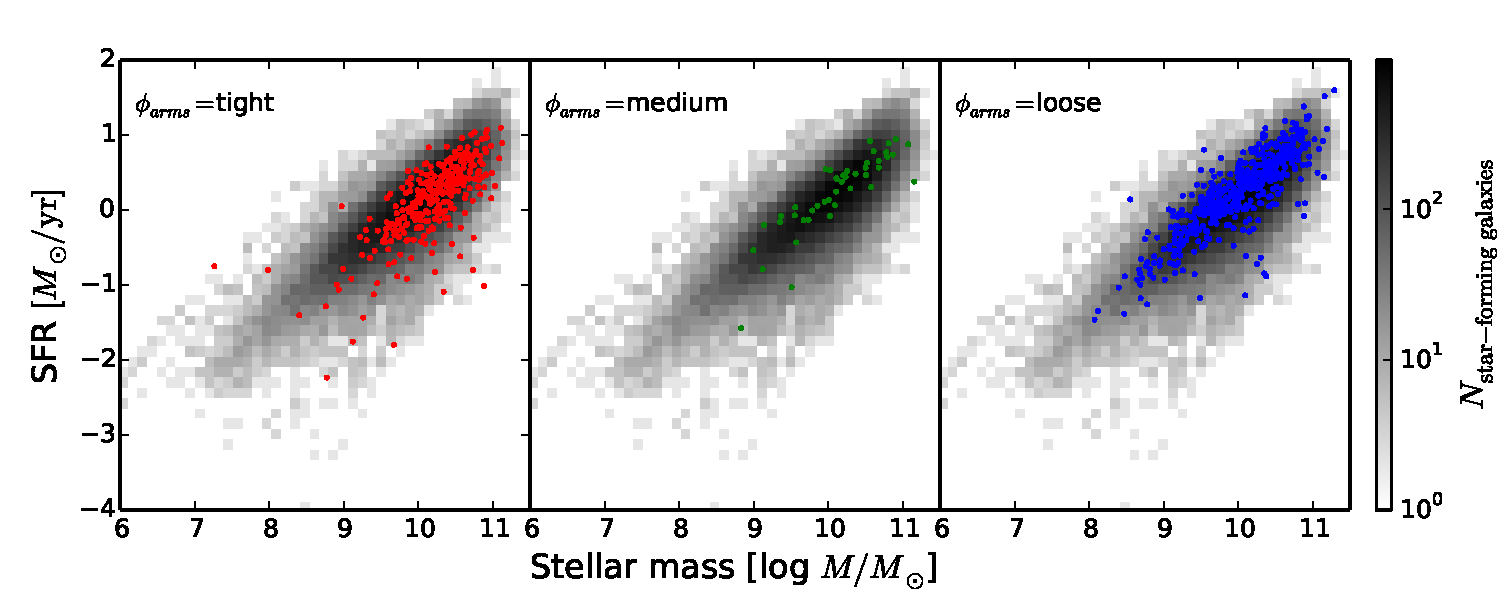
\includegraphics[angle=0,width=7.0in]{figures/ms_arms_winding.pdf}
\caption{Total star formation rate as a function of stellar mass; grayscale colors are the same as in Figure~\ref{fig-number}. From left to right: red, green, and blue points are spiral galaxies with ``tight'', ``medium'', and ``loose'' winding spiral arms as identified by GZ2 morphology flags. Dotted lines show the weighted least-squares linear fit as split by pitch angle; the solid line is the fit to all star-forming galaxies. 
\label{fig-winding}}
\end{figure*}

It should also be noted that the galaxies in GZ2 flagged as a function of pitch angle are not representative of the true vote distribution. The raw numbers in Figure~\ref{fig-winding} suggest that most spiral galaxies are either tightly or loosely wound. In fact, the plurality classification for most galaxies is for medium-winding; the spread in votes is typically large, though, and so users rarely agree on the medium option at the 80\% level which sets the flag. Plotting the same star-forming main sequence diagram as a function of $p_{\rm medium}$, which more accurately tracks the pitch angle distribution, also closely follows the main star-forming main sequence. % Figure ms_arms_winding_weighted_pmed.pdf shows this. 

\begin{figure*}
%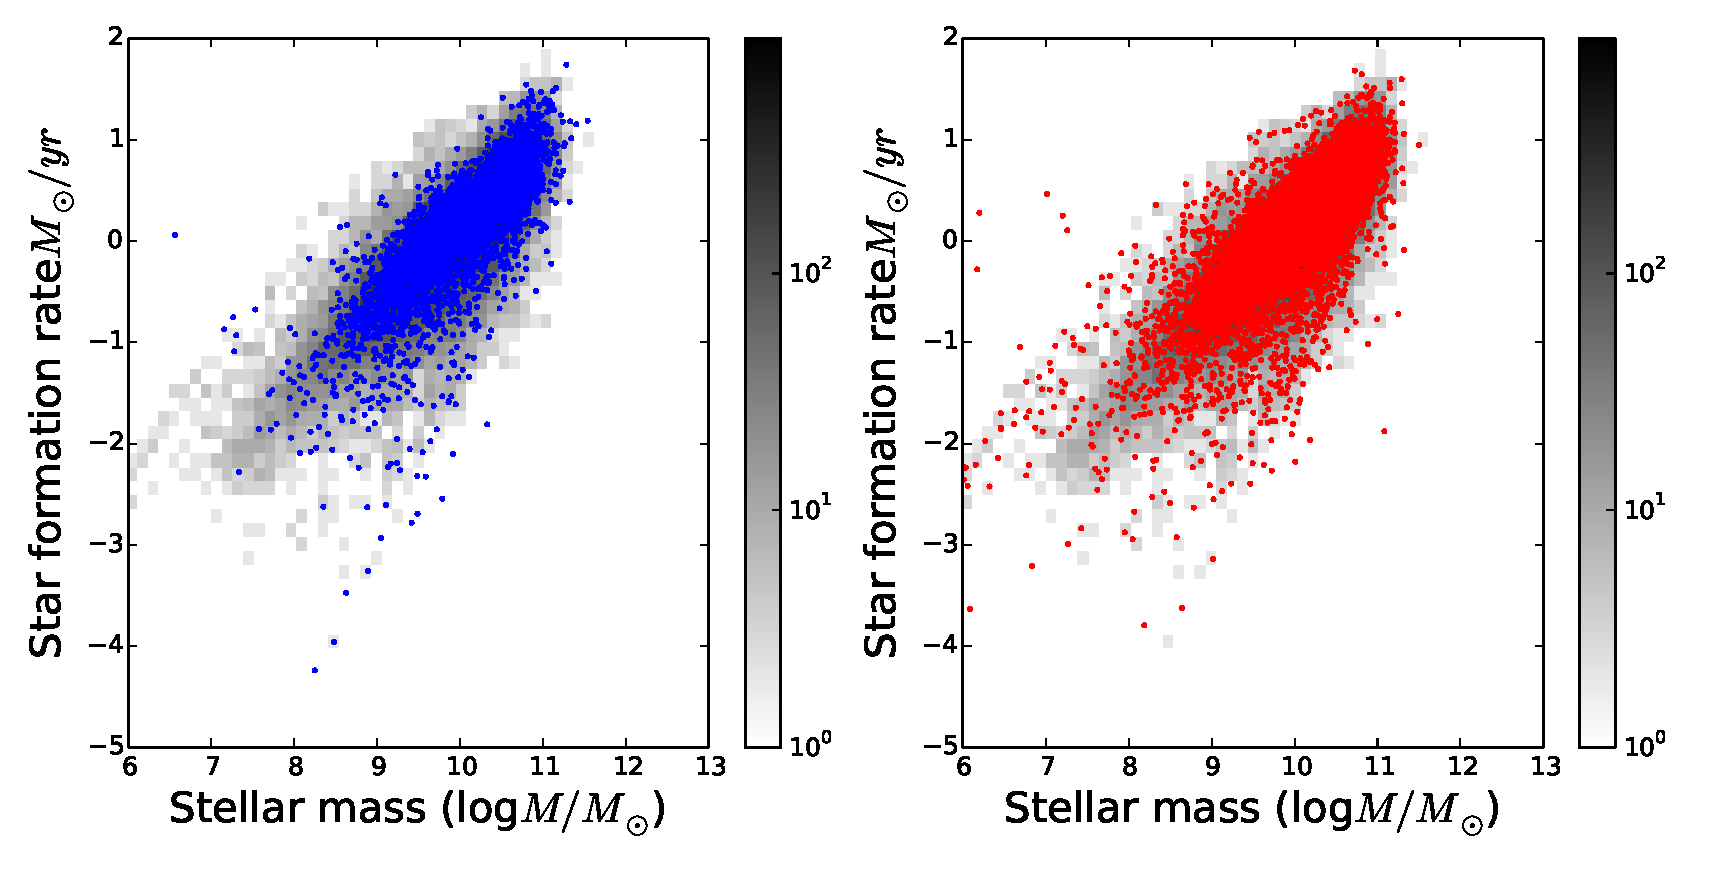
\includegraphics[angle=0,width=7.0in]{figures/ms_bar.pdf}
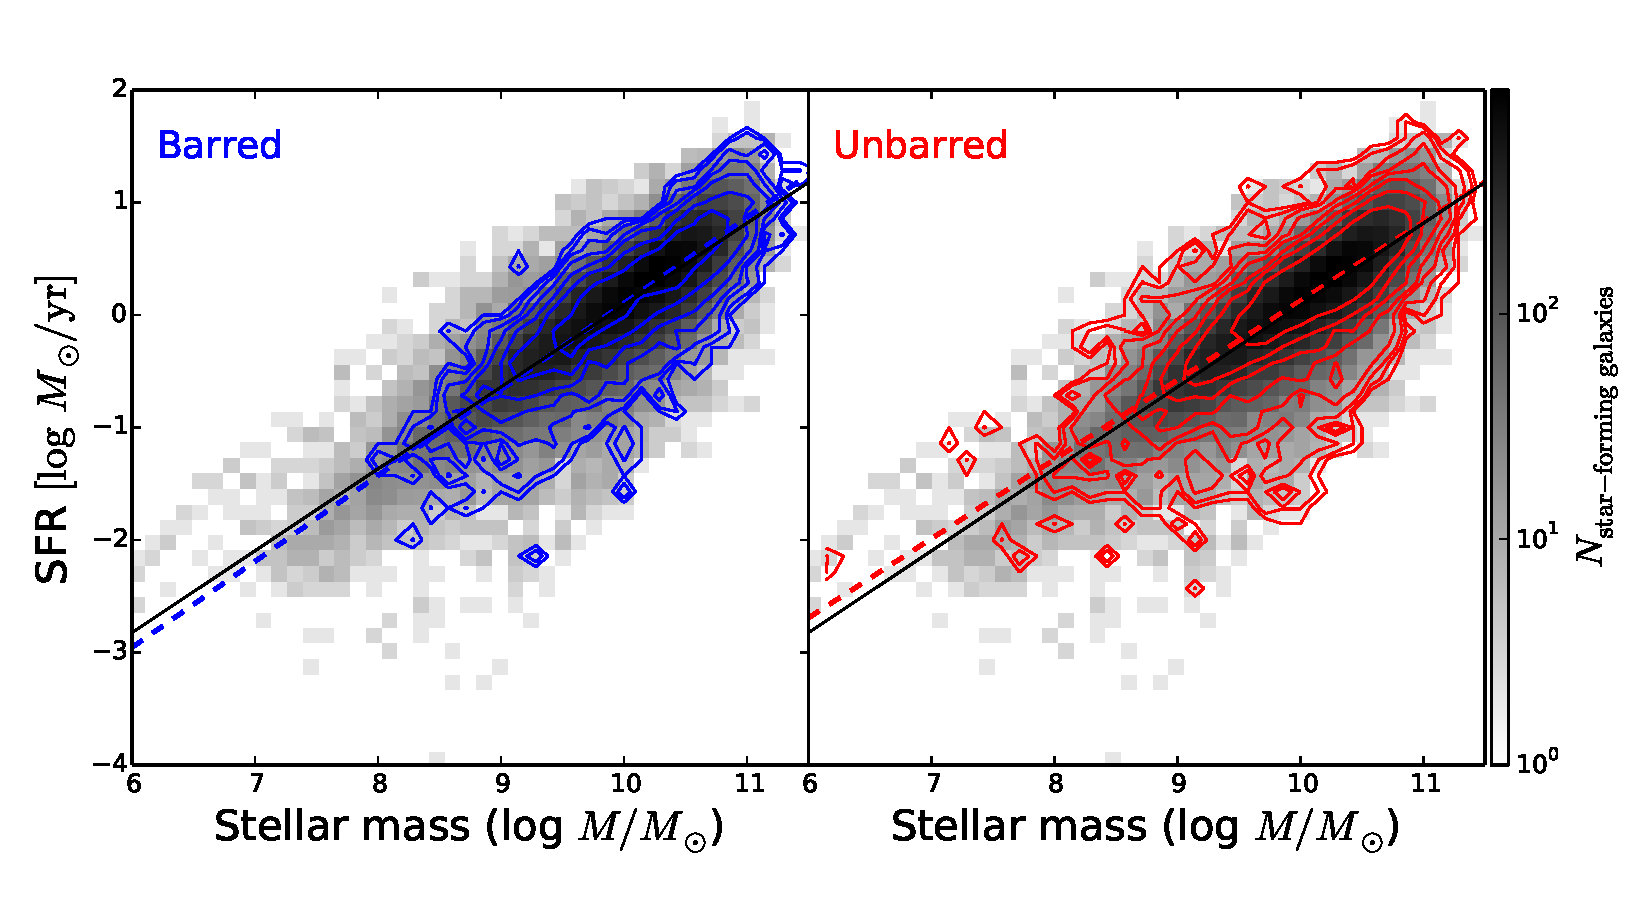
\includegraphics[angle=0,width=7.0in]{figures/ms_bar_contour.pdf}
\caption{Total star formation rate as a function of stellar mass; grayscale colors are the same as in Figure~\ref{fig-number}. Left: blue contours show the distribution of barred galaxies ($p_\textrm{bar}\ge0.4$ for previously-identified disks) from GZ2. Right: red contours are the distribution of remaining disk galaxy population with no evidence for a strong bar ($p_\textrm{bar}<0.4$). Dotted lines show the weighted least-squares linear fit to the barred/unbarred population; the solid line is the fit to all star-forming galaxies. 
\label{fig-bar}}
\end{figure*}

Finally, we examine the effect of a large-scale galactic bar on the star-forming main sequence. This sample is significantly larger than those including spiral arm morphology, since the classification is at a higher level in the GZ2 tree and has only two choices; this results in a higher percentage of consensus classifications that set the flag. Figure~\ref{fig-bar} shows the star-forming main sequence for both barred and unbarred galaxies. Although the fraction of barred galaxies potentially varies as a function of stellar mass \citep{mas11c}, both the linear fits and ranges of the sub-populations are consistent with all star-forming galaxies. In other words, the presence of a bar does not affect the galaxy's position on the star-forming main sequence. 

%%%%%%%%%%%%
%%% DISCUSSION
%%%%%%%%%%%%

\section{Discussion}\label{sec-discussion}

\begin{figure*}
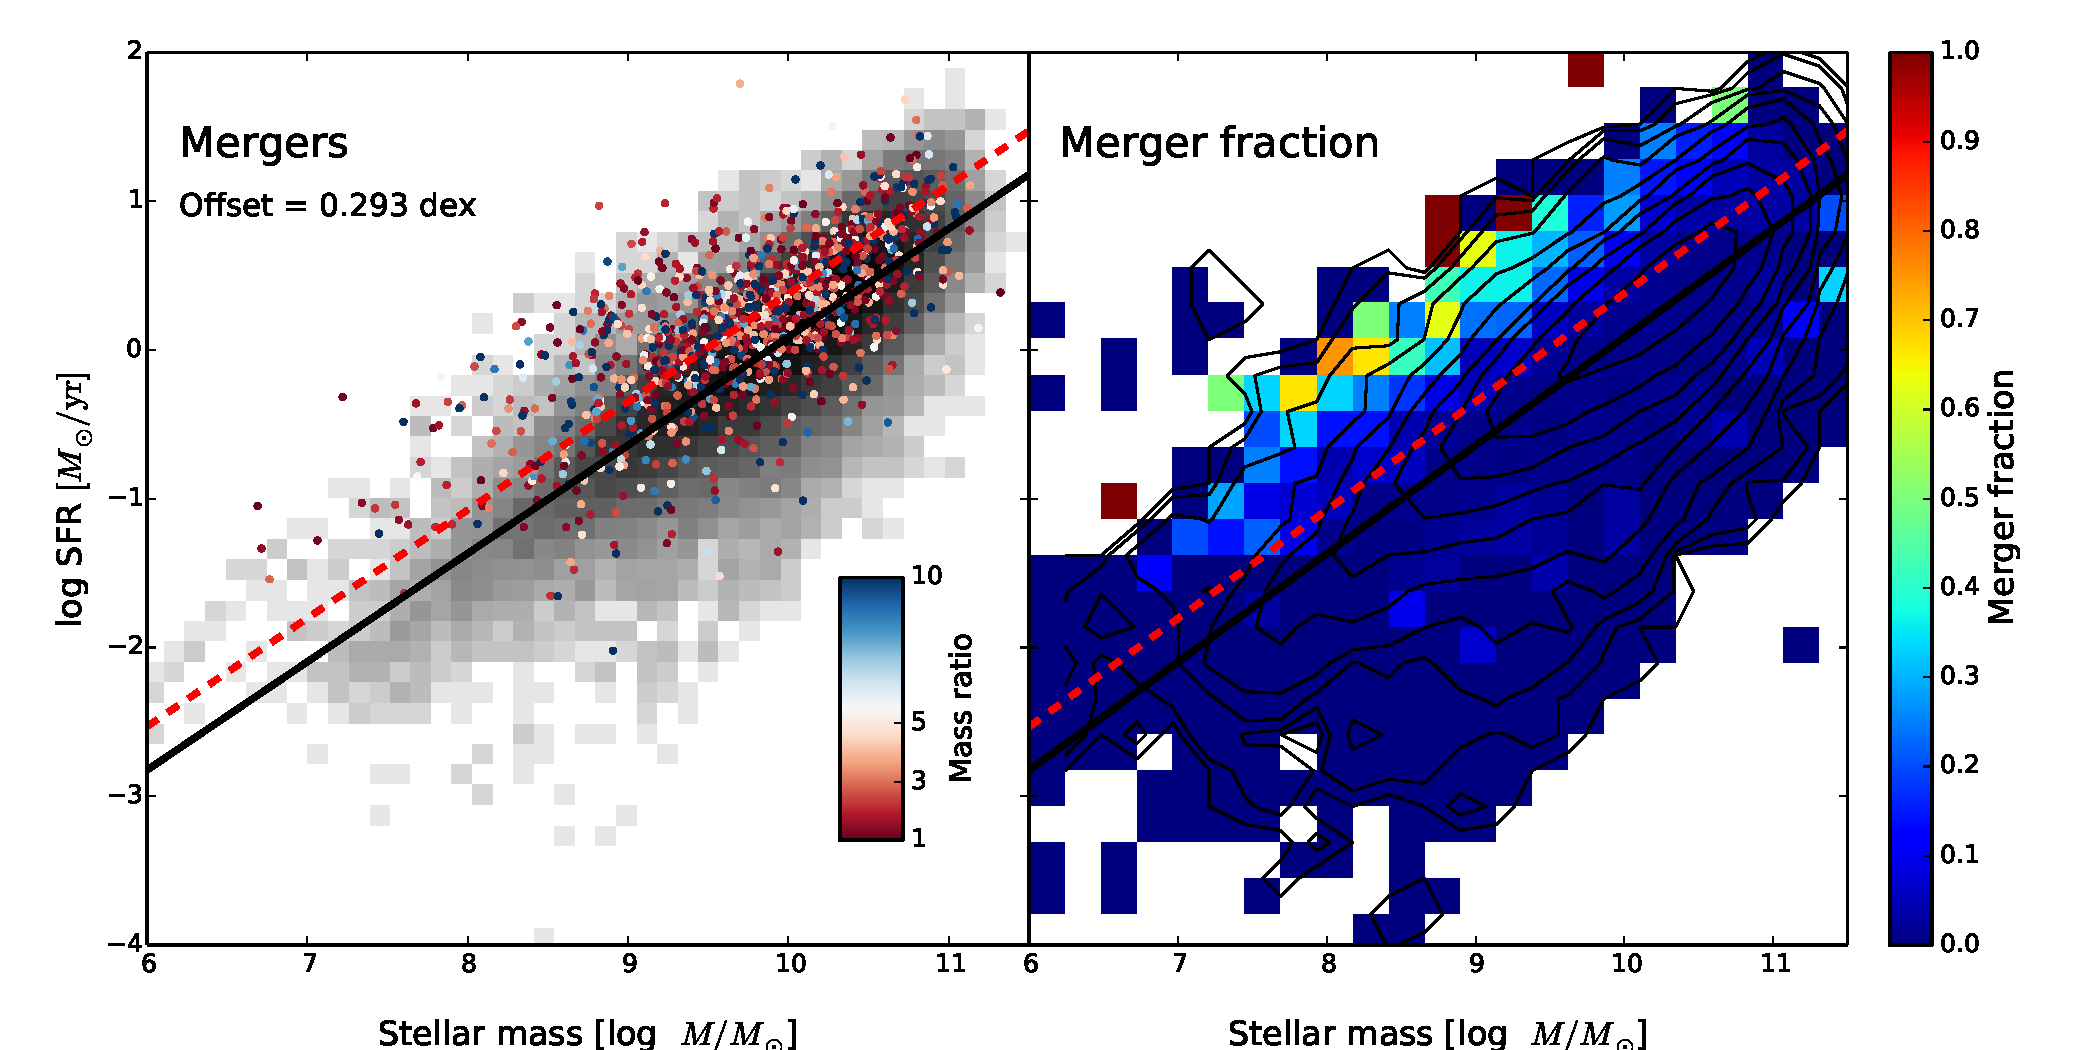
\includegraphics[angle=0,width=7.0in]{figures/ms_mergers_both.pdf}
\caption{Total star formation rate as a function of stellar mass; grayscale colors are the same as in Figure~\ref{fig-number}. Left: Coloured points show 2,978~merging galaxies from \citet{dar10a}. Mergers are colour-coded by the mass ratio of the primary and secondary galaxies; there is no clear difference in the merging populations with regard to the SFMS when comparing major to minor mergers. When fixing the slope of the star-forming main sequence and allowing the offset to vary, mergers (dotted line) have higher SFRs by $\sim0.3$~dex compared to all star-forming galaxies (solid line). Right: Star-forming galaxies binned and colour-coded by merger fraction ($N_\textrm{mergers}/N_\textrm{star-forming galaxies})$. Overplotted lines are the same as left plot. Of the galaxies that lie furthest above the SFMS, more than $50\%$ are unambiguous mergers. 
\label{fig-mergers}}
\end{figure*}

Our results show that the star-forming main sequence is remarkably robust to the details of the spatial distribution of star formation \textit{within} galaxies. Testing for a wide range of morphological sub-types of star-forming disk galaxies yields no statistically significant difference in the relative position of these sub-types vis-\'a-vis the main sequence. Neither the number or pitch angle of spiral arms, or the presence of a large-scale bar are correlated with any detectable increase or decrease in the efficiency of star formation. The system which regulates star formation in galaxies is thus either not affected by the details of the spatial distribution of star formation, or its regulatory effect is so strong that it wipes out any such effect in a short time. 

The agreement of all sub-varieties of star-forming galaxies is supported by the close agreement to the linear fits to the data for all well-sampled categories (Table~\ref{tbl-fits}). This tracks only the slope and offset of the distribution, however, and not its width. We thus also compared the sample standard deviation ($\sigma_{SFR}$) as a function of mass of the star-forming galaxy population to its various subsamples. The value of $\sigma_{SFR}$ monotonically decreases with mass over the range $6.0<\log(M/M_\odot)<11.5$. For all populations examined in this paper, though, the widths of their distributions are consistent with the broader population. % Figure to be shown in Appendix?

\citet{abr14} found that by normalizing galaxies by the stellar mass of the disk alone, the slope of the SFMS is consistent with only a linear trend (removing any dependence on mass). Although this correction to the disk stellar mass homogenizes the SFMS for disks with a range of $B/T$, the dispersion ($\sigma_{SFR}$) of the sequence must be a result of contributions by bars, disk dynamics, halo heating, AGN activity, and/or environment (among other factors). Our results show that the neither of the first two factors play dominant roles in controlling $\sigma_{SFR}$, at least as far as major dynamical drivers (such as strong bars or additional arms) are concerned. Thus while the overall bulge strength does affect the position of a galaxy on the SFMS \citep{mar09,lan14,oma14}, the structure of the \emph{disk itself} does not.

The lack of any difference in SFR as a function of mass for barred vs. unbarred galaxies is in general agreement with \citet{ell11}, who find an increase of $\Delta~\textrm{SFR}\sim0.15$~dex, but only for galaxies with $M_\star>10^{10.7}~M_\odot$. This is at the very upper end of the mass range probed in Figure~\ref{fig-bar}. If the increase in star formation is limited to the central kpc of the disk (as they demonstrate using fibre SFR measurements), an increase in possible bar-driven SFR increase is seen down to $M_\star=10^{10}~M_\odot$. 

Amongst individual galaxies that lie significantly off the SFMS, compact starburst galaxies show the largest increase in SFR at a given mass \citep{elb11}. In the local Universe, these include optically-identified ``green pea'' galaxies, which have unusually high sSFR and can lie more than 1~dex above the SFMS \citep{car09}. While few known green pea galaxies have detailed imaging available, their most common morphology is in a clumpy arrangement with knots of bright star formation. There is thus little evidence for a dynamically-settled disk (in any arrangment) for galaxies in the local Universe lying significantly above the SFMS. 

As a comparison to the kpc-scale structures discussed above, we analyze the impact of the most significant forcing event to a galaxy system known -- a major galaxy merger (Figure~\ref{fig-mergers}). In these systems (which are in various stages of coalescence) the star formation rates are increased by only an average of 0.29~dex, corresponding to less than a factor of two overall. \citet{dar10} showed that in the local ($z<0.1$) Universe, galaxies with intense bursts of star formation are limited to only the spiral (disc) galaxies. This increase in star formation for mergers does show a strong evolution in redshift out to at least $1.5<z<2.5$, likely due to the higher gas fractions involved \citep{dad10,rod11}. 

The location of mergers on the present-day SFMS shows just how stable the regulatory system in galaxies really is. Almost all simulations of galaxy mergers predict a steep increase in the star formation rate during both first passage and final coalescence \citep[eg,][]{hop08}. The magnitude of this increase often depends on the details of the simulation, but can range from a factor of 10 to 100. In the low-redshift universe sampled by SDSS and Galaxy~Zoo, we find no evidence for an enhancement of such magnitude. This in turn suggests that the current generation of galaxy merger simulations misses critical feedback mechanisms that prevent runaway peaks in star formation rates during mergers.

\section{Conclusions}

We analyze for the first time the detailed structure of disks in star-forming galaxies as related to their position on the $M_\star$-SFR relation, using morphological classifications from the Galaxy~Zoo~2 project. We find that neither the slope nor the dispersion of the star-forming galaxies are affected when splitting the sample into different categories of disks, including barred/unbarred galaxies, the pitch angle of spiral arms, or the number of spiral arms. 

The uniformity of disk galaxies along the SFMS, regardless of their kpc-scale structure, argues for the system as a whole being strongly self-regulated. While smaller regions of the galaxy can experience (likely temporary) increases in star formation, the amount of star formation in the disk as a whole is conserved. This is preserved even for the strongest forcing events, including major mergers; the physics governing the SFMS are primarily driven by the overall mass of the system. This means that simulations of galaxy evolution must be able to meet the challenge of simultaneously reproducing the wide range of disk morphologies observed along the Hubble sequence (and in various merger stages) while simultaneously managing feedback so that \emph{all} disk types maintain the same tight relationship to the SFMS.

%%%%%%%%%%%%
%%% ACKNOWLEDGMENTS
%%%%%%%%%%%%

\acknowledgments

The data in this paper are the result of the efforts of the Galaxy~Zoo volunteers, without whom none of this work would be possible. Their efforts are individually acknowledged at \url{http://authors.galaxyzoo.org}. Please contact the authors to request access to research materials discussed in this paper. 

We thank Rory Smith and Lucio Mayer for useful discussions. This research made use of TOPCAT, an interactive graphical viewer and editor for tabular data \citep{tay05}. 
%The development of Galaxy Zoo 2 was supported by The Leverhulme Trust. KWW and LFF would like to acknowledge support from the US National Science Foundation under grant DRL-0941610. CJL acknowledges support from the Science and Technology Facilities Council (STFC) Science in Society program. KS gratefully acknowledges support from Swiss National Science Foundation Grant PP00P2\_138979/1. TM acknowledges funding from the STFC ST/J500665/1. RCN was partially supported by STFC grant ST/K00090X/1. BDS acknowledges support from Worcester College, Oxford, and from the Oxford Martin School program on computational cosmology.

KS gratefully acknowledges support from Swiss National Science Foundation Grant PP00P2\_138979/1.

Funding for the SDSS and SDSS-II has been provided by the Alfred P. Sloan Foundation, the Participating Institutions, the National Science Foundation, the U.S. Department of Energy, the National Aeronautics and Space Administration, the Japanese Monbukagakusho, the Max Planck Society, and the Higher Education Funding Council for England. The SDSS website is \url{http://www.sdss.org/}.

The SDSS is managed by the Astrophysical Research Consortium for the Participating Institutions. The Participating Institutions are the American Museum of Natural History, Astrophysical Institute Potsdam, University of Basel, University of Cambridge, Case Western Reserve University, University of Chicago, Drexel University, Fermilab, the Institute for Advanced Study, the Japan Participation Group, Johns Hopkins University, the Joint Institute for Nuclear Astrophysics, the Kavli Institute for Particle Astrophysics and Cosmology, the Korean Scientist Group, the Chinese Academy of Sciences (LAMOST), Los Alamos National Laboratory, the Max-Planck-Institute for Astronomy (MPIA), the Max-Planck-Institute for Astrophysics (MPA), New Mexico State University, Ohio State University, University of Pittsburgh, University of Portsmouth, Princeton University, the United States Naval Observatory, and the University of Washington.

%%%%%%%%%%%%
%%% BIBLIOGRAPHY
%%%%%%%%%%%%

\bibliography{kwrefs}

\end{document}


